% book example for classicthesis.sty
\documentclass[10pt,paper=a4 BCOR0, DIV15, titlepage=false, oneside]{scrbook} % KOMA-Script book
\usepackage[T1]{fontenc}                
\usepackage{lipsum}
\usepackage[linedheaders,parts,pdfspacing]{classicthesis} % ,manychapters
%\usepackage[osf]{libertine}
\usepackage{amsthm}
\usepackage[T1]{fontenc}
\usepackage[utf8]{inputenc}
\usepackage{polski}
\usepackage{graphicx}
\usepackage{geometry}
\newgeometry{tmargin=2.5cm, bmargin=1.5cm, lmargin=1.5cm, rmargin = 1.5cm}
\renewcommand{\contentsname}{Instrukcja obsługi programu Mopnik}
\begin{document}
%	\pagestyle{scrheadings}
% \manualmark
%	\markboth{\spacedlowsmallcaps{\contentsname}}{\spacedlowsmallcaps{\contentsname}}	
\tableofcontents 
%\automark[section]{chapter}
%	\renewcommand{\chaptermark}[1]{\markboth{\spacedlowsmallcaps{#1}}{\spacedlowsmallcaps{#1}}}
%	\renewcommand{\sectionmark}[1]{\markright{\thesection\enspace\spacedlowsmallcaps{#1}}}

    % use \cleardoublepage here to avoid problems with pdfbookmark
    %\cleardoublepage\part{Widok po uruchomieniu programu}
    \chapter*{Widok po uruchomieniu programu}
    \addtocounter{chapter}{1}
    \addcontentsline{toc}{chapter}{Widok po uruchomieniu programu}
    \section{Wyświetlanie mapy}
    \paragraph{}
    Po uruchomieniu programu ładowane są domyślne dane:
    \begin{enumerate}
    \item Kafelki mapy w formacie graficznym (służą one tylko wizualizacji).
    \item Mapa sieci drogowej w formacie OSM.
    \item Dane dotyczące średniodobowego natężenia ruchu (pochodzące z
      Generalnego Pomiaru Ruchu w 2015r.
      \footnote{\url{https://www.gddkia.gov.pl/userfiles/articles/g/generalny-pomiar-ruchu-w-2015_15598//SYNTEZA/WYNIKI_GPR2015_DK.pdf}}
    \item Dane dotyczące rozmieszczenia MOP-ów.
    \end{enumerate}
 \begin{figure}[ht]
      \centering
      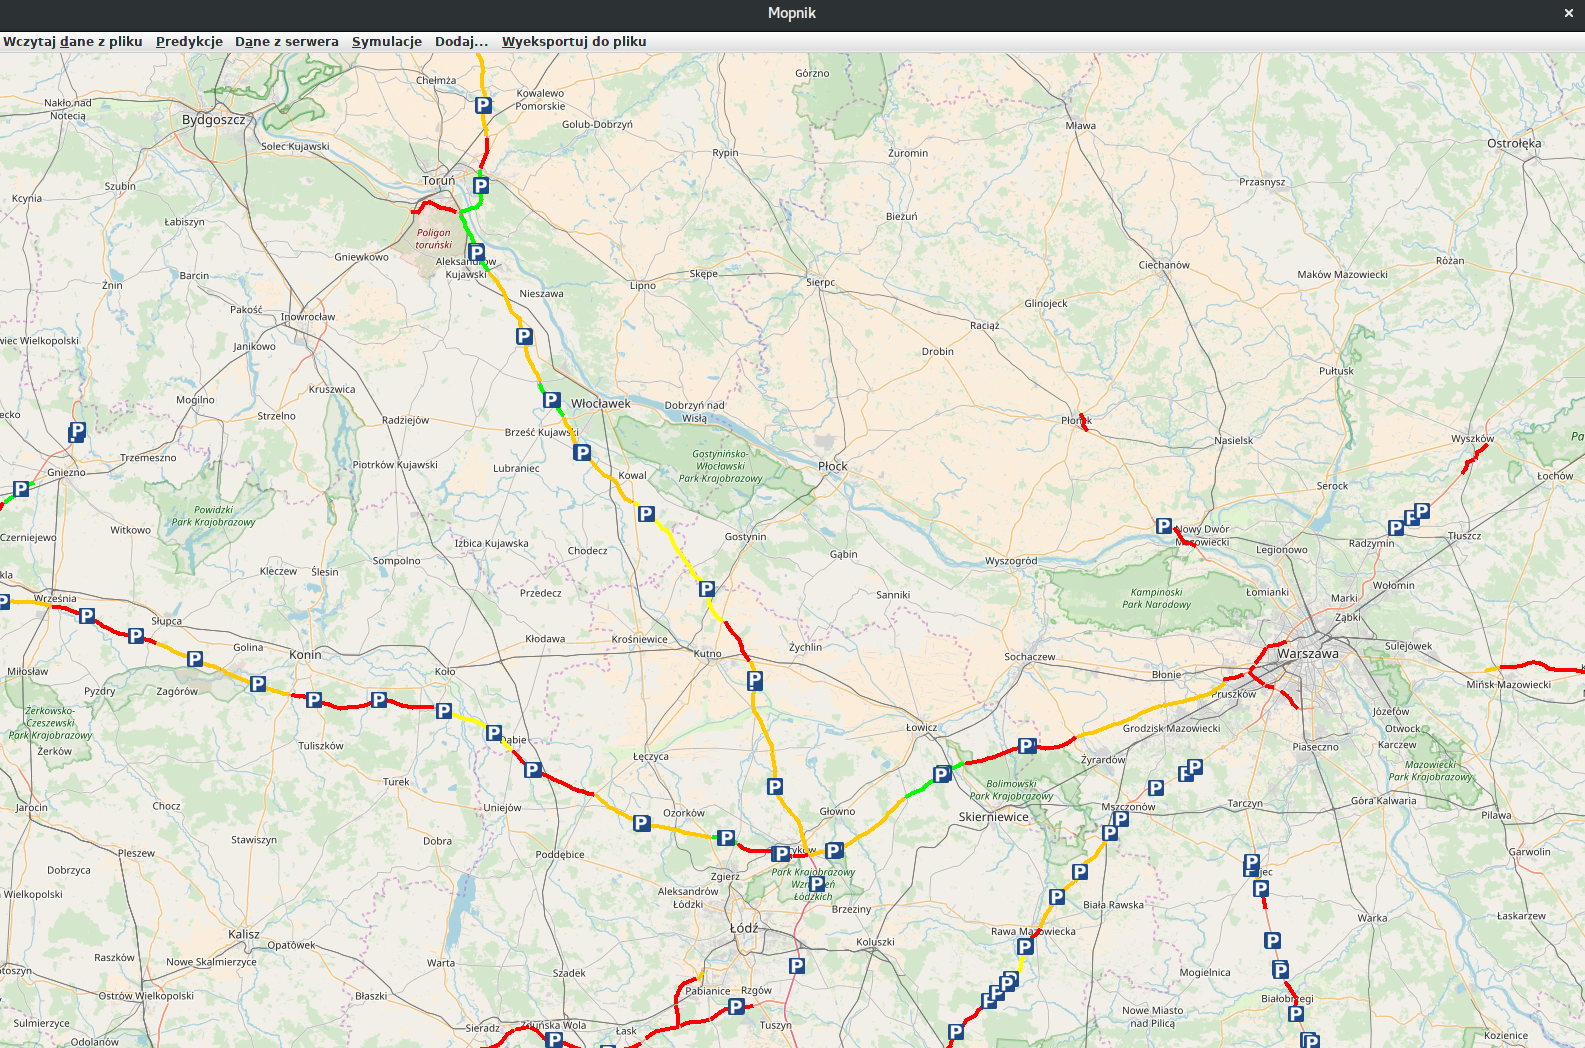
\includegraphics[width=\textwidth]{widok_glowny.png}
      \caption{Widok główny po uruchomieniu programu}
    \end {figure}
    
    Oprócz tego domyślnie jest ustawiona metodyka przewidywania potrzebnych
    miejsc parkingowych pochodząca z pracy Malwiny Spławińskiej i Katarzyny
    Soleckiej
    \footnote{\url{http://www.autobusy-test.com.pl/images/stories/Do_pobrania/2017/nr\%2012/Bezp\%20i\%20ekol/073_013_A_BiE_SPLAWINSKA_SOLECKA.pdf}}.
        Wraz z parametrami zaproponowanymi w tej metodyce.

    Na podstawie tych danych, dla poszczególnych odcinków dróg (ekspresowych i
    autostrad) są wyliczane istniejące oraz potrzebne liczby miejsc
    parkingowych. Są one zaznaczane na mapie kolorami w następujący sposób:
    \begin{itemize}
      \item Kolorem zielonym są zaznaczone te odcinki, gdzie liczba miejsc
        parkingowych jest wystarczająca, a dla niektórych typów pojazdów nawet
        zbyt wysoka.
      \item Kolorem żółtym są zaznaczone te odcinki, gdzie liczba miejsc jest
        wystarczająca (tzn. liczba miejsc wg. metodyki $\ge$ liczba istniejących
        miejsc).
      \item Kolorem pomarańczowym są zaznaczone te odcinki, gdzie brakuje
        miejsc dla pewnego typu pojazdu w co najmniej jednym kierunku.
      \item Kolorem czerwonym są zaznaczone te odcinki, gdzie brakuje miejsca
        dla większości typów pojazdów w obu kierunkach.
     \end{itemize}

        \section{Oglądanie danych}
      Możliwe jest również oglądanie szczegółowych danych dotyczących
      konkretnych MOP-ów oraz konkretnych odcinków sieci drogowej. Po
      kliknięciu w interesującego nas MOP-a lub drogę wyświetla się okno
      dialogowe zawierające m.in. następujące informacje (por. rysunki 2 i 3):
      \begin{itemize}
        \item Dla MOP-a:
          \begin{itemize}
            \item Podstawowe dane takie jak droga, pikietaż, kierunek, oddział.
            \item Liczba miejsc parkingowych dla pojazdów konkretnego typu.
            \item Infrastruktura (stacja benzynowa, toaleta, restauracja itd.).
          \end{itemize}
        \item Dla odcinka drogi:
          \begin{itemize}
            \item Nazwa drogi oraz pikietaż początku i końca.
            \item Średniodobowe natężenie ruchu na tym odcinku.
            \item Liczba potrzebnych (wg. domyślnej metodyki) oraz liczba
              istniejących w rzeczywistości (suma po MOP-ach stojących przy
              danym odcinku) miejsc parkingowych. Podzielona ze względu na
              kierunek i typ pojazdu.
          \end{itemize}
      \end{itemize}
      \begin{figure}[ht]
        \centering
       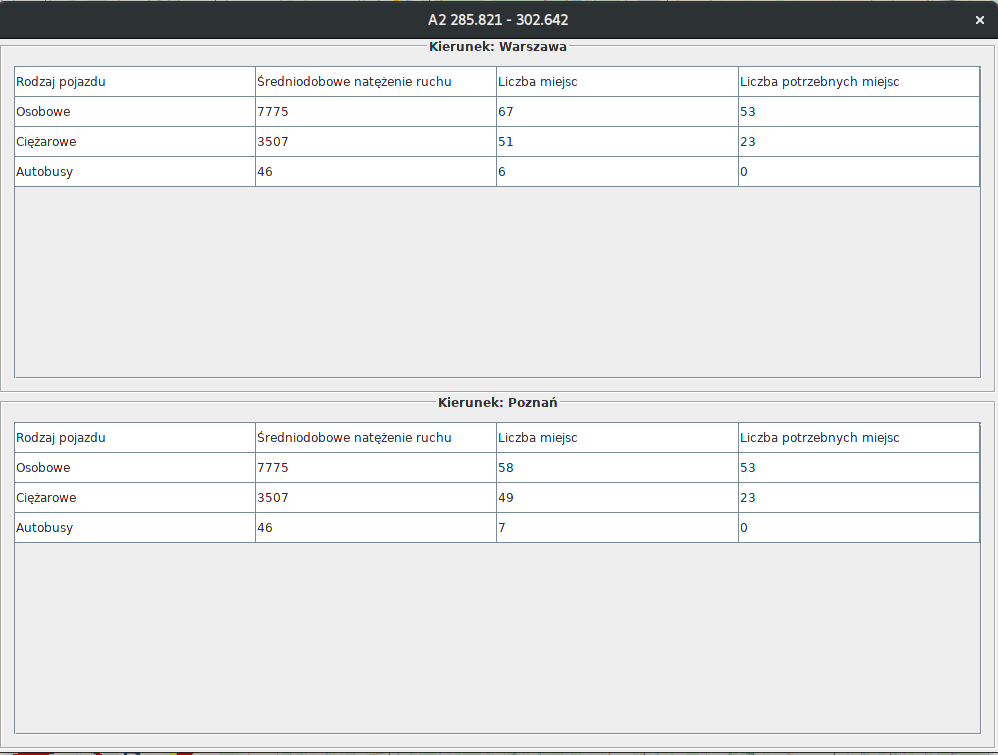
\includegraphics[width=.8\textwidth]{podglad_drogi.png}
        \caption{Podgląd odcinka drogi}
      \end{figure}
      \begin{figure}[ht]
          \centering
          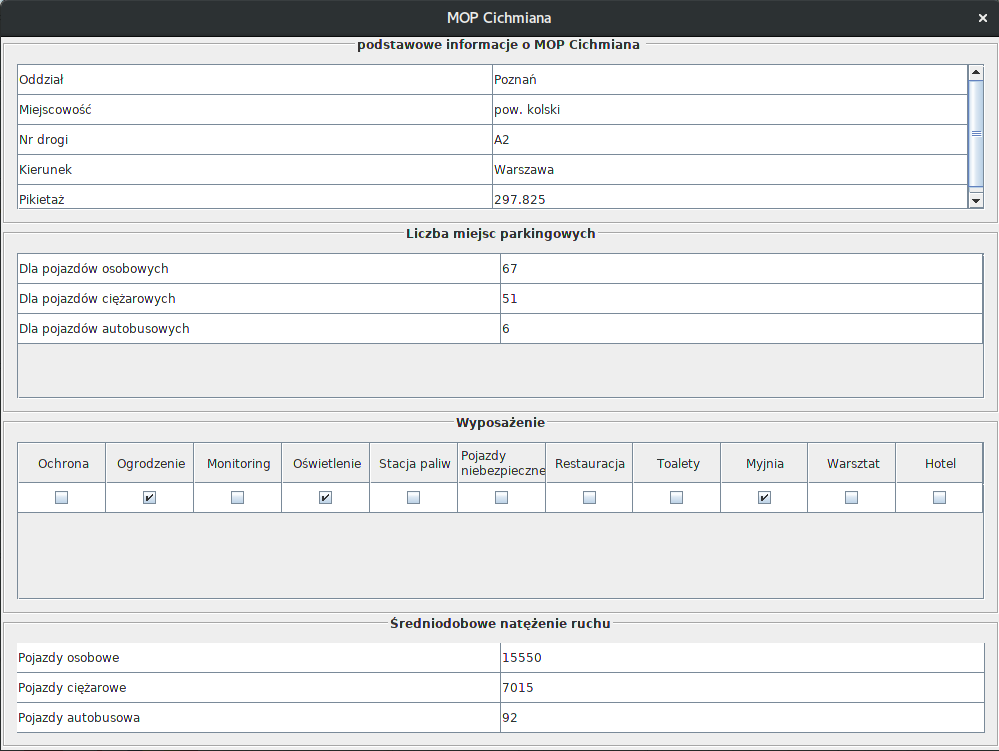
\includegraphics[width=.8\textwidth]{podglad_mopa.png}
          \caption{Podgląd MOP-a}
      \end{figure}

      \chapter*{Modyfikacja danych}
      \addcontentsline{toc}{chapter}{Modyfikacja danych}
      \addtocounter{chapter}{1}
      \setcounter{section}{0}

      Możliwa jest zmiana domyślnych danych. Po ich wprowadzeniu, wyniki
      natychmiast są obliczane ponownie i zaznaczanie na mapie.

      \section{Parametry metodyki}
        Aby zmienić domyślne parametry metodyki należy z głównego menu wybrać
        Predykcje > Zajętości MOP-ów > Domyślna metodyka. Pojawi się okienko z
        parametrami. Dwukrotne kliknięcie na wartość daje możliwość edycji. Po
        kliknięciu przycisku \textit{Ustaw parametry} zmiany będą widoczne na
        mapie.

      \section{Średniodobowe natężenie ruchu}
        Aby dodać dane dotyczące średniodobowego natężenia ruchu należy z
        głównego menu wybrać Wczytaj dane z pliku > Średniodobowe natężenie
        ruchu. Wczytywany plik musi być w formacie csv, jeden rząd na jeden
        odcinek drogi. Kolejność pól powinna być taka, jak ta w GPR2015 czyli następująca:
        \begin{enumerate}
          \item Numer punktu pomiarowego
          \item Numer drogi (kraj)
          \item Numer drogi (E)
          \item Pikietaż początku (kilometry i metry oddzielone przecinkiem)
          \item Pikietaż końca (kilometry i metry oddzielone przecinkiem)
          \item Długość
          \item Nazwa
          \item SDR pojazdów silnikowych ogółem 
          \item SDR ze względu na rodzaj pojazdu, kolejno:
          \begin{itemize}
            \item Motocykle
            \item Samochody osobowe i mikrobusy
            \item Samochody dostawcze
            \item Samochody ciężarowe bez przyczepy
            \item Samochody ciężarowe z przyczepą
            \item Autobusy 
          \end{itemize}
        \end{enumerate}
        Plik nie powinien też zawierać nagłówka z tytułami kolumn. Dodanie
        pliku w złym formacie nie powiedzie się.

        \section{Układ MOP-ów}
        \subsection{Z pliku w formacie json} TODO
        \subsection{Z serwera} TODO

        \chapter*{Dodawanie nowych obiektów}
        \setcounter{section}{0}
        \addcontentsline{toc}{chapter}{Dodawanie nowych obiektów}
        \addtocounter{chapter}{1}
        \section{Drogi}
        W celu dodania nowego odcinka drogi, należy z głównego menu wybrać
        Dodaj... > Drogę. Następnie wybrać dwa punkty na mapie, gdzie ma być
        początek i koniec drogi. Kolejność kliknięć ma znaczenie -- pierwsze
        będzie oznaczało początek, drugie koniec. Następnie należy wypełnić
        okienko odpowiednimi wartościami (jak na rysunku poniżej). 

       \begin{figure}[ht]
        \centering
       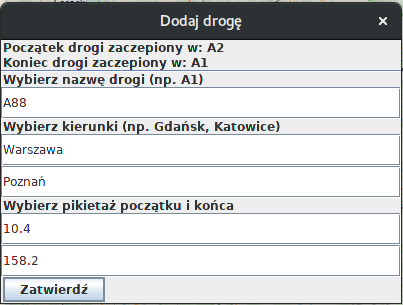
\includegraphics[width=.3\textwidth]{dodawanie_drogi.png}
        \caption{Dodawanie drogi}
      \end{figure}

      \section{MOP-a}
      W celu dodania nowego MOP-a należy z głównego menu wybrać Dodaj... >
      MOP-a. Następnie wybrać punkt na mapie, gdzie ma być umieszczony MOP.
      Jeżeli punkt jest wystarczająco blisko istniejącej (lub dodanej) drogi,
      zostanie do niej przypisany. W tym wypadku należy również wybrać kierunek
      -- a więc stronę drogi, przy której MOP ma stanąć. Po zatwierdzeniu tych
      danych, w odpowiednim miejscy mapy pojawia się czerwona ikonka
      oznaczająca dodanego MOP-a. Dane dotyczące liczby miejsc parkingowych i
      wyposażenia można edytować w jego podglądzie. Zmiana liczby miejsc
      parkingowych spowoduje ponowne obliczenie liczby miejsc przy odpowiednim
      odcinku drogi i ewentualną zmianę kolorów na mapie. 

     \begin{figure}[ht]
       \begin{minipage}{.3\textwidth}
        \centering
       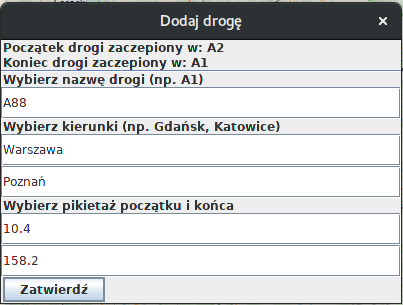
\includegraphics[width=.9\linewidth]{dodawanie_drogi.png}
        \caption{Dodawanie MOP-a}
      \end{minipage}%
      \begin{minipage}{.6\textwidth}
        \centering
       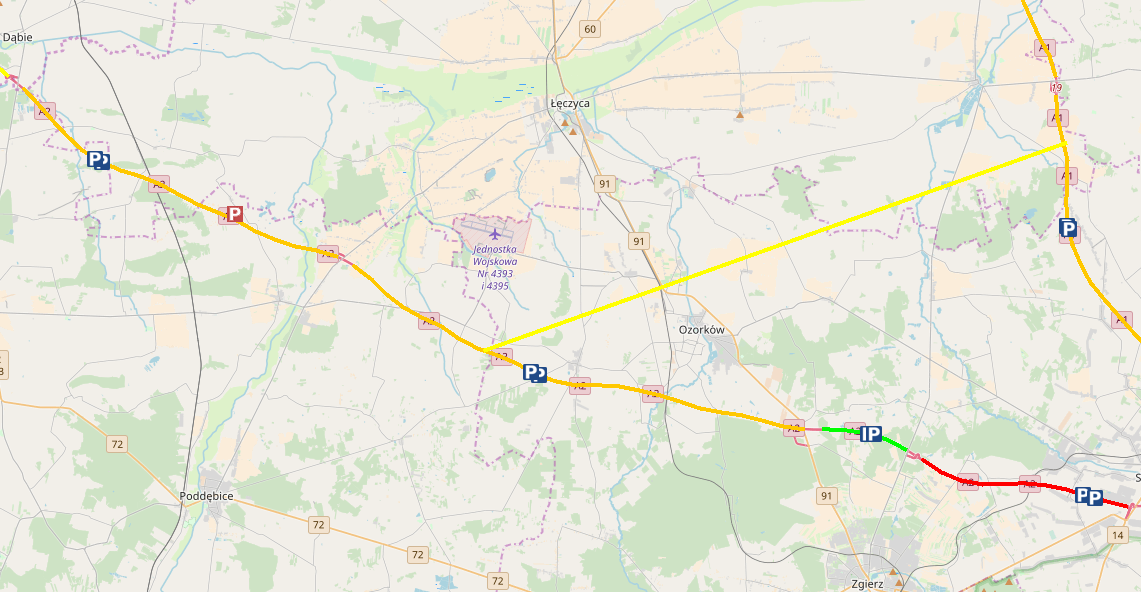
\includegraphics[width=.9\linewidth]{dodany_mop_droga.png}
        \caption{Mapa z nowym MOP-em i nową drogą}
      \end{minipage}
      \end{figure}


    \chapter*{Symulacje}
    \addtocounter{chapter}{1}
    \setcounter{section}{0}
    \addcontentsline{toc}{chapter}{Symulacje}
    TODO

    \chapter*{Zapisywanie danych do pliku}
    \addtocounter{chapter}{1}
    \setcounter{section}{0}
    \addcontentsline{toc}{chapter}{Zapisywanie danych do pliku}

    \section{Układ MOPów}

  




\end{document}





